\documentclass[10pt, xcolor = svgnames, aspectratio=43]{beamer} %Beamer
\usepackage{palatino} %font type
\usefonttheme{metropolis} %Type of slides
\usefonttheme[onlymath]{serif} %font type Mathematical expressions
\usetheme[progressbar = frametitle,titleformat frame=smallcaps,numbering=counter]{metropolis} %This adds a bar at the beginning of each section.
\useoutertheme[subsection=false]{miniframes} %Circles in the top of each frame, showing the slide of each section you are at

\usepackage{appendixnumberbeamer} %enumerate each slide without counting the appendix
\setbeamercolor{progress bar}{fg=Maroon!70!Coral} %These are the colours of the progress bar. Notice that the names used are the svgnames
\setbeamercolor{title separator}{fg=DarkSalmon} %This is the line colour in the title slide
\setbeamercolor{structure}{fg=black} %Colour of the text of structure, numbers, items, blah. Not the big text.
\setbeamercolor{normal text}{fg=black!87} %Colour of normal text
\setbeamercolor{alerted text}{fg=DarkRed!60!Gainsboro} %Color of the alert box
\setbeamercolor{example text}{fg=Maroon!70!Coral} %Colour of the Example block text


\setbeamercolor{palette primary}{bg=NavyBlue!50!DarkOliveGreen, fg=white} %These are the colours of the background. Being this the main combination and so one. 
\setbeamercolor{palette secondary}{bg=NavyBlue!50!DarkOliveGreen, fg=white}
\setbeamercolor{palette tertiary}{bg=NavyBlue!40!Black, fg= white}
\setbeamercolor{section in toc}{fg=NavyBlue!40!Black} %Color of the text in the table of contents (toc)

%These next packages are the useful for Physics in general, you can add the extras here. 
\usepackage{amsmath, amssymb}
\usepackage{slashed}
\usepackage[superscript, ref]{cite}
\usepackage{relsize}
\usepackage{caption}
\usepackage{subcaption}
\usepackage{multicol}
\usepackage{booktabs}
\usepackage[scale=2]{ccicons}
\usepackage{pgfplots}
\usepgfplotslibrary{dateplot}
\usepackage{geometry}
\usepackage{xspace}
\usepackage[useregional]{datetime2}
\usepackage{fancybox}
\usepackage{romannum}
\usepackage{hyperref}
\usepackage{siunitx}
\usepackage{listings}
\usepackage{color}
\usepackage{framed}
\usepackage[strict]{changepage}




\definecolor{dkgreen}{rgb}{0,0.6,0}
\definecolor{gray}{rgb}{0.5,0.5,0.5}
\definecolor{mauve}{rgb}{0.58,0,0.82}

\lstset{frame=tb,
  language=FORTRAN,
  aboveskip=3mm,
  belowskip=3mm,
  showstringspaces=false,
  columns=flexible,
  basicstyle={\small\ttfamily},
  numbers=none,
  numberstyle=\tiny\color{gray},
  keywordstyle=\color{blue},
  commentstyle=\color{dkgreen},
  stringstyle=\color{mauve},
  breaklines=true,
  breakatwhitespace=true,
  tabsize=4
}

%\usepackage[super, square]{natbib}

\newcommand{\themename}{\textbf{\textsc{bluetemp}\xspace}}%metropolis}}\xspace}


\newcommand{\TEX}[0]{
\includegraphics[height = 9.5pt]{./logos/TeX.pdf}}
\newcommand{\LATEX}[0]{\includegraphics[height = 9.5pt]{./logos/LATeX.pdf}}
\newcommand{\FORTRAN}[0]{
\includegraphics[height = 9.5pt]{./logos/Fortran.pdf}}
\newcommand{\PYTHON}[0]{
\includegraphics[height = 9.5pt]{./logos/Python.pdf}}
\newcommand{\MMA}[0]{
\includegraphics[height = 9.5pt]{./logos/Mathematica.pdf}}
\newcommand{\CERN}[0]{
\includegraphics[height = 9.5pt]{./logos/CERN_ROOT.pdf}}
\newcommand{\GPT}[0]{
\includegraphics[height = 9.5pt]{./logos/GPT.pdf}}
\newcommand{\TORCH}[0]{
\includegraphics[height = 9.5pt]{./logos/Torch.pdf}}
\newcommand{\NUMBA}[0]{
\includegraphics[height = 9.5pt]{./logos/Numba.pdf}}
\newcommand{\CC}[0]{
\includegraphics[height = 9.5pt]{./logos/cc.pdf}}
\newcommand{\ALL}[0]{\FORTRAN\PYTHON\MMA}

\renewcommand\citeform[1]{[#1]}

% environment derived from framed.sty: see leftbar environment definition
\definecolor{formalshade}{rgb}{0.95,0.95,1}
\definecolor{mygray}{gray}{0.4}
\definecolor{lightgray}{gray}{0.93}

\newenvironment{formal}{%
  \def\FrameCommand{%
    \hspace{1cm}%  ← change this to modify the indentation ========================
    {\color{mygray}\vrule width 2pt}%
    {\color{lightgray}\vrule width 4pt}%
    \colorbox{lightgray}%
  }%
  \MakeFramed{\advance\hsize-\width\FrameRestore}%
  \noindent\hspace{-4.55pt}% disable indenting first paragraph
  \begin{adjustwidth}{}{7pt}%
  \vspace{2pt}\vspace{2pt}%
}
{%
  \vspace{2pt}\end{adjustwidth}\endMakeFramed%
}



\title{Computer Programming\\on Geosciences}
\author[Name]{Gauss Chang\inst{$\dagger$}}
\subtitle{N-body Simulation}


\institute[uni] % (optional)
{
	\inst{\dagger}
	Department of Physics \\
	\textsc{National Taiwan University}
}


% \date{\today} %Here you can change the date
\date{\DTMdate{2024-12-17}} %Here you can change the date

\titlegraphic{\vspace{0.0cm}\hfill
\includegraphics[width = 1.3in]{./logos/NTU.pdf}}

\begin{document}
{
\setbeamercolor{background canvas}{bg=NavyBlue!50!DarkOliveGreen, fg=white}
\setbeamercolor{normal text}{fg=white}
\maketitle
}%This is the color of the first slide. bg= background and fg=foreground

\metroset{titleformat frame=smallcaps} %This changes the titles for small caps




%\begin{frame}{Outline}
%  \setbeamertemplate{section in toc}[sections numbered]
%  \tableofcontents[hideallsubsections]
%\end{frame}
\begin{frame}{Outline}
	\begin{columns}[t]
		\begin{column}{0.5\textwidth}
			\setbeamertemplate{section in toc}[sections numbered]
			\tableofcontents[sections={1-4},hideallsubsections]
		\end{column}
		\begin{column}{0.5\textwidth}
			\setbeamertemplate{section in toc}[sections numbered]
			\tableofcontents[sections={5-8},hideallsubsections]
		\end{column}
	\end{columns}
\end{frame}



\section{Background}


\begin{frame}{Background: Inspiration}
\begin{figure}
\shadowbox{
\centering

\includegraphics[height=1.7in]{../fig/scz.jpeg}}
\end{figure}
\end{frame}



\begin{frame}[fragile]{Background: $N$-Body Problem}
\begin{minipage}{0.45\textwidth}
The n-body problem seeks to predict the motions of a group of celestial objects interacting gravitationally.

It involves determining their interactive forces and true orbital trajectories over time, given their initial positions, velocities, and other properties.
\end{minipage}
\hspace{20pt}
\begin{minipage}{0.45\textwidth}
\begin{figure}
\shadowbox{
\centering
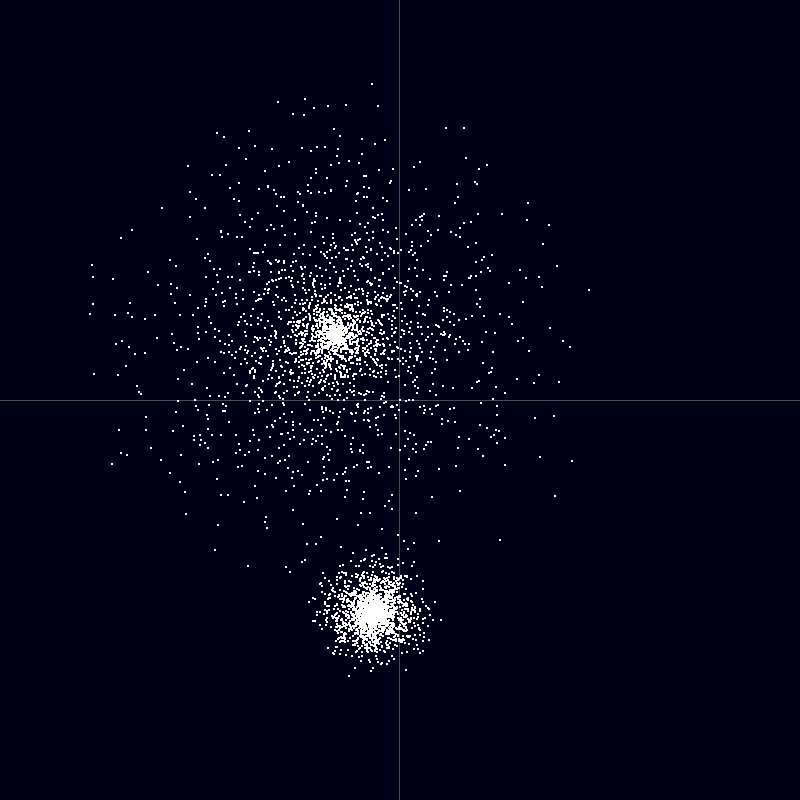
\includegraphics[width = 0.8\textwidth]{../fig/Barnes_hut_partikel.png}}
\caption{The N body problem.}
\label{The-N-body-problem}
\end{figure}
\end{minipage}
\end{frame}


\begin{frame}{Background: $N$-Body Problem}
\begin{itemize}
	\item Classical Mechanics: Focuses on celestial dynamics like planetary motion and star clusters, using Newtonian physics.
	\item General Relativity: Adds complexity by considering spacetime distortions caused by massive objects.
	\item Applications: Includes understanding the solar system, star clusters, and galaxy dynamics.
	\item Simplified Cases: The restricted three-body problem is a notable special case.
	\item Solving the n-body problem often requires numerical simulations due to the lack of general analytical solutions.
\end{itemize}
\end{frame}



\section{Algorithm}


\begin{frame}{Algorithm: Newton's Law of Gravitation}
\begin{align}
	\mathbf{F}
	& = \frac{G m_1 m_2}{\left| \mathbf{r_1} - \mathbf{r_2} \right|^3} (\mathbf{r_1} - \mathbf{r_2})
\end{align}
\begin{itemize}
    \item $G$: Gravitational constant
    \item $m_1, m_2$: Masses of the two bodies
    \item $\mathbf{r_1}, \mathbf{r_2}$: Position vectors of the bodies
    \item The force $\mathbf{F}$ exerted on $m_1$ by $m_2$ is attractive and along the line connecting the two masses.
    \item Elastic Collision.
\end{itemize}
\end{frame}



\begin{frame}[fragile]{Algorithm: Barnes--Hut Algorithm\cite{barnes_hierarchical_1986}}
\begin{minipage}{0.65\textwidth}
\begin{itemize}
    \item \textbf{Motivation:} Direct $N$-body simulations are $O(N^2)$, which is costly for large $N$.
    \item \textbf{Key Idea:} 
    \begin{itemize}
        \item Use a hierarchical spatial decomposition (quadtree in 2D, octree in 3D).
        \item Group distant particles into cells and approximate their collective influence by a single mass located at their center of mass.
        \item Elastic Collision
    \end{itemize}
\end{itemize}
\end{minipage}
\hspace{20pt}
\begin{minipage}{0.25\textwidth}
\begin{figure}
\shadowbox{
\centering
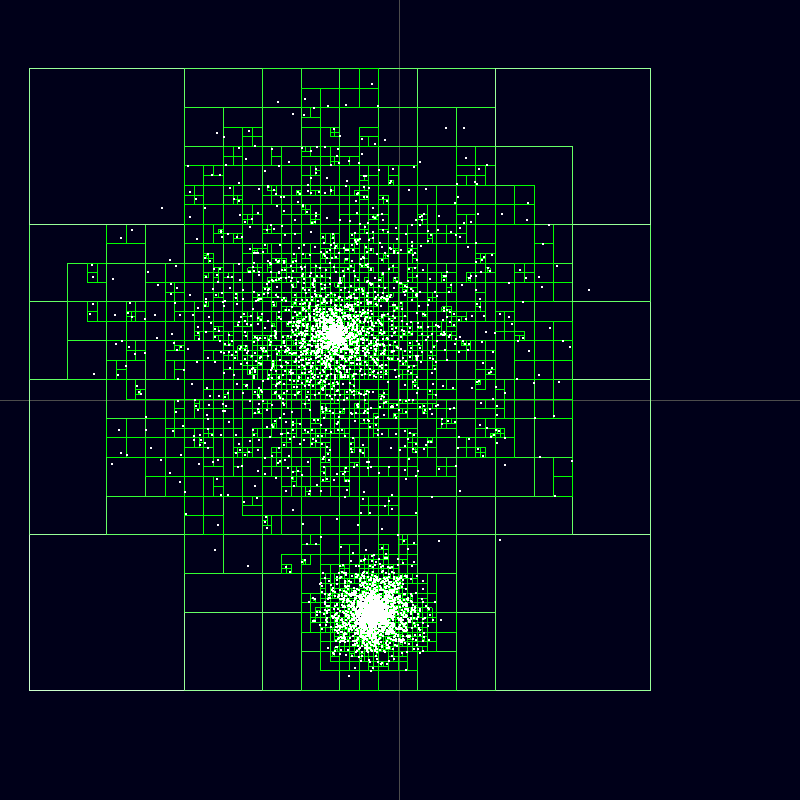
\includegraphics[width = 0.9\textwidth]{../fig/Barnes_hut_tree.png}}
\caption{Barnes–Hut tree.}
\label{Barnes–Hut-tree}
\end{figure}
\end{minipage}
\end{frame}


\begin{frame}{Algorithm: Barnes--Hut Algorithm}
\begin{figure}
\shadowbox{
\centering
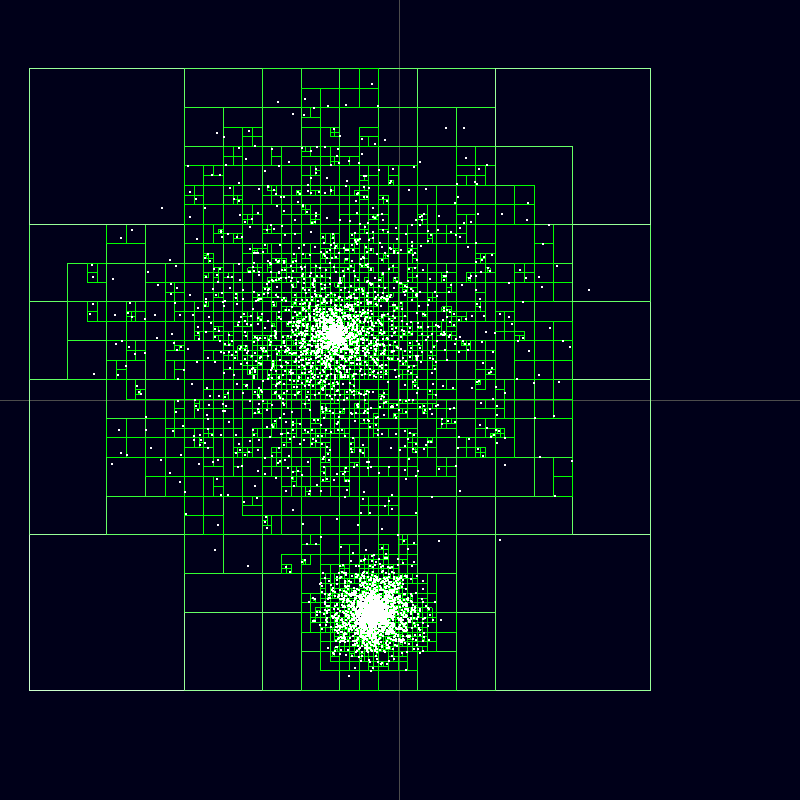
\includegraphics[height=2.6in]{../fig/Barnes_hut_tree.png}}
\caption{Barnes–Hut tree (2D).}
\label{Barnes–Hut-tree2}
\end{figure}
\end{frame}

\begin{frame}{Algorithm: Barnes--Hut Algorithm}
\begin{figure}
\shadowbox{
\centering
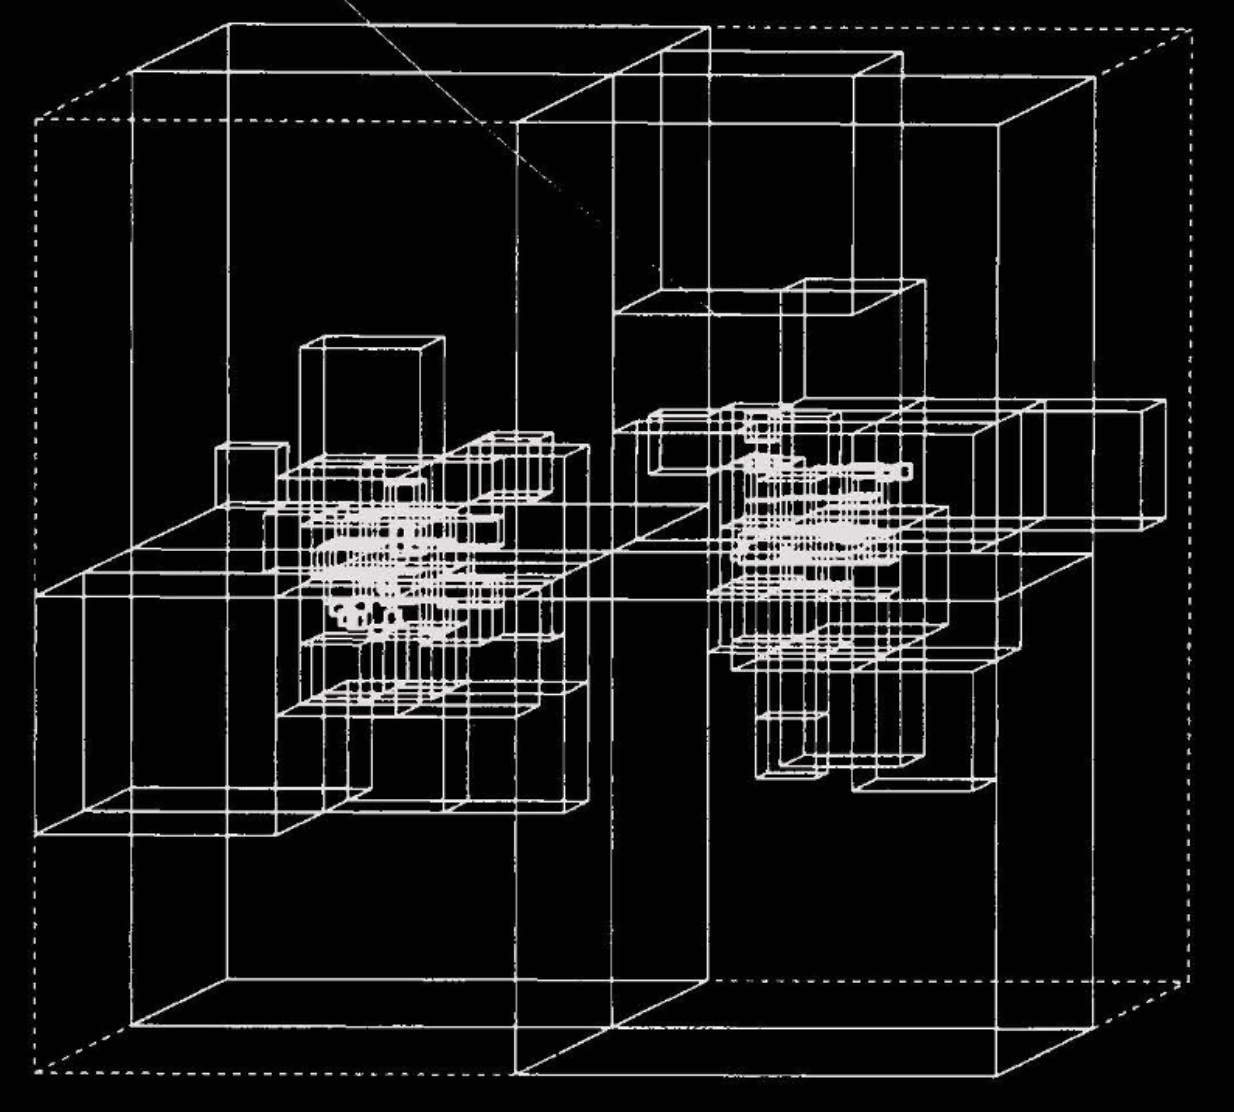
\includegraphics[height=2.55in]{../fig/Barnes_hut_tree2}}
\caption{Barnes–Hut tree (3D).\cite{barnes_hierarchical_1986}}
\label{Barnes–Hut-tree3}
\end{figure}
\end{frame}





\begin{frame}{Algorithm: Barnes--Hut Algorithm}
\begin{enumerate}
    \item \textbf{Build the Tree:}
    \begin{itemize}
        \item Start with the entire simulation domain as the root.
        \item Recursively subdivide the domain into smaller cells until each leaf node contains only a few particles.
    \end{itemize}
    \item \textbf{Compute Mass Properties:}
    \begin{itemize}
        \item For each node, compute total mass and center of mass of all particles in its subtree.
    \end{itemize}
    \item \textbf{Force Calculation:}
    \begin{itemize}
        \item For a given particle, traverse the tree.
        \item If a node is sufficiently "far away," approximate all its particles by the node's center of mass.
        \item Otherwise, descend into its children for finer resolution.
    \end{itemize}
\end{enumerate}
\end{frame}

\begin{frame}{Algorithm: Direct $N$-Body vs. Barnes--Hut}
\begin{itemize}
    \item \textbf{Direct $N$-Body Simulation:}
    \begin{itemize}
        \item Complexity: $O(N^2)$
        \item Each particle interacts directly with every other particle.
        \item Provides high accuracy but is computationally expensive.
    \end{itemize}
    
    \item \textbf{Barnes--Hut Approximation:}
    \begin{itemize}
        \item Complexity: $O(N \log N)$ on average
        \item Trades a small loss in accuracy for a significant gain in efficiency.
        \item Accuracy can be tuned via the opening angle $\theta$: 
        a smaller $\theta$ means more accuracy but higher cost.
    \end{itemize}
\end{itemize}
\end{frame}


\begin{frame}{Algorithm: Time Integration}


\begin{itemize}
	\item Simple `Euler method', which updates the position and velocity for a given particle by \textit{timestep} $\Delta t$ via
	\begin{align}
		\mathbf{x} \left( t + \Delta t \right)
		& = \mathbf{x} \left( t \right) + \mathbf{\dot x} \left( t \right) \cdot \Delta t \\
		\mathbf{\dot x} \left( t + \Delta t \right)
		& = \mathbf{\dot x} \left( t \right) + \mathbf{\ddot x} \left( t \right) \cdot \Delta t
	\end{align}
	
	\item From the Taylor expansion of the position and its time derivatives at time $t + \Delta t$
	\begin{align}
		\mathbf{x_1}
		& = \mathbf{x_0} + \frac{1}{2} \left( \mathbf{\dot x_0} + \mathbf{\dot x_1} \right) \Delta t + \frac{1}{12} \left( \mathbf{a_0} - \mathbf{a_1} \right) \Delta t^2 + O \left( \Delta t^5 \right) \\
		\mathbf{\dot x_1}
		& = \mathbf{\dot x_0} + \frac{1}{2} \left( \mathbf{a_0} + \mathbf{a_1} \right) \Delta t + \frac{1}{12} \left( \mathbf{\dot a_0} - \mathbf{\dot a_1} \right) \Delta t^2 + O \left( \Delta t^5 \right)
	\end{align}
\end{itemize}


\end{frame}







\section{Simulation Setup}


\begin{frame}[fragile]{Simulation Setup: Initial Condition}
Generate N particle randomly.
\begin{itemize}
	\item Mass is randomly assigned between $1 \sim 2$.
	\item Position ($r_x, r_y, r_z$) is randomly assigned between $- \frac{L}{2} \sim \frac{L}{2}$.
	\item Velocity ($v_x, v_y, v_z$) is randomly assigned between $-1 \sim 1$.
	\item Radius ($r$) is randomly assigned between $0.001 \sim 0.05$.
	\item No initial acceleration.
\end{itemize}
\end{frame}


\begin{frame}{Simulation Setup: Initial Condition}
\begin{figure}
\shadowbox{
\centering
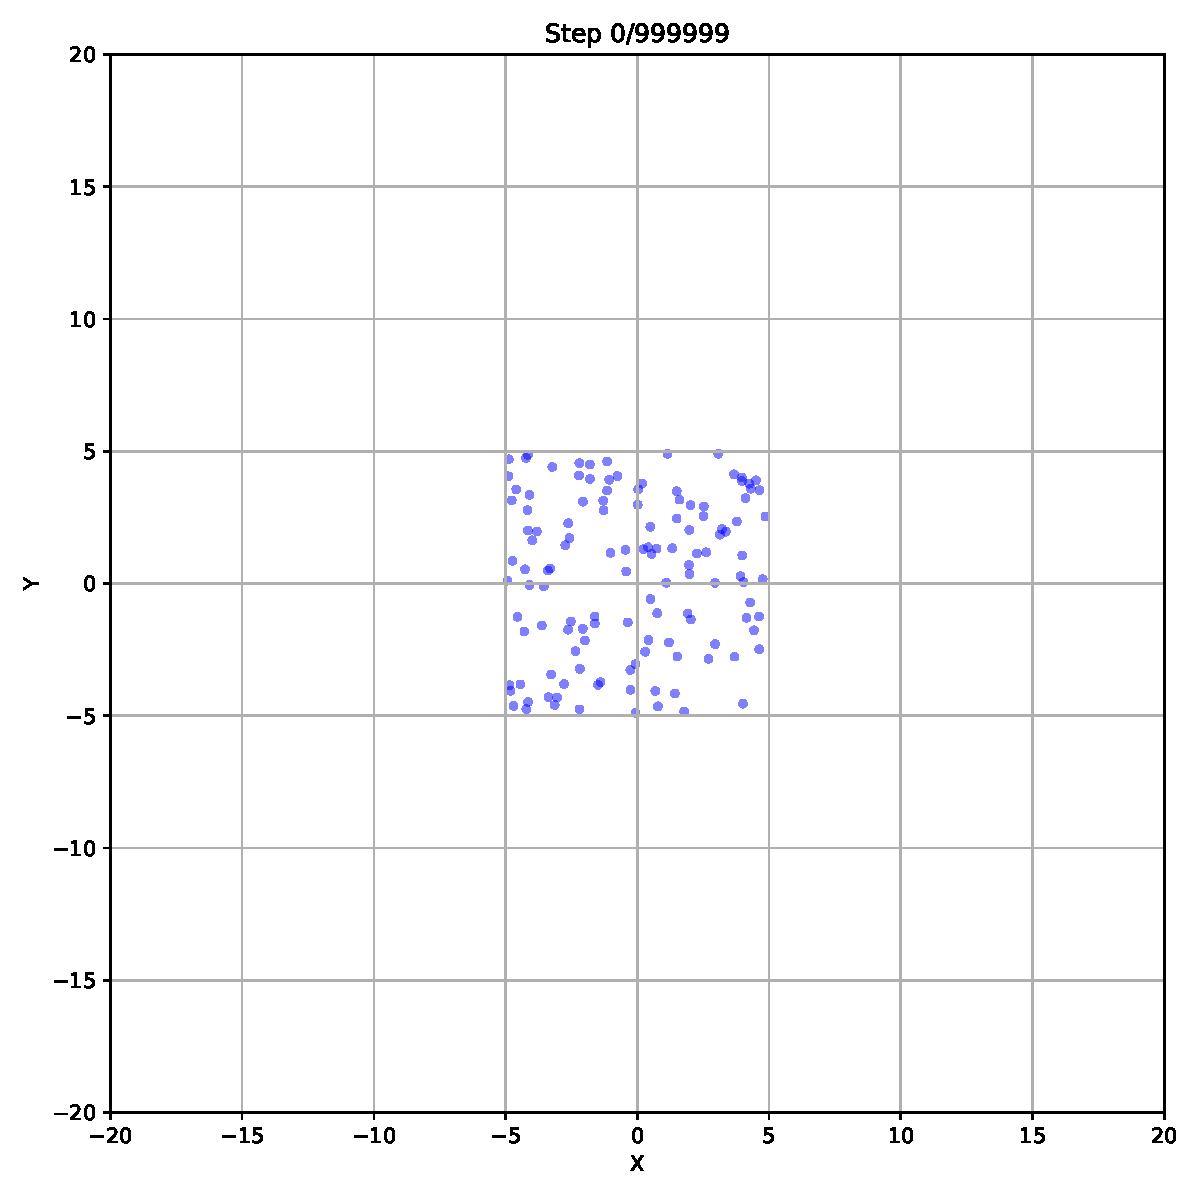
\includegraphics[height=2.6in]{../plot/step_0.pdf}}
\caption{Initial particle distribution.}
\label{Initial-particle-distribution}
\end{figure}
\end{frame}







\section{Results}



\begin{frame}{Results: Metrics for Evaluate Simulation Results}

I use the two conservation laws to check if the simulation has broken.

\begin{itemize}
	\item Conservation of total energy, $\sum E = \sum \left( T + V \right) $ of the system.
	\item Conservation of total angular Momentum, $\sum \mathbf{L}$.
\end{itemize}

Record $\sum E$ and $\sum \mathbf{L}$ in every simulation step, and plot against time.
\end{frame}



\begin{frame}{Results: Energy v.s. Time}
\begin{figure}
\shadowbox{
\centering
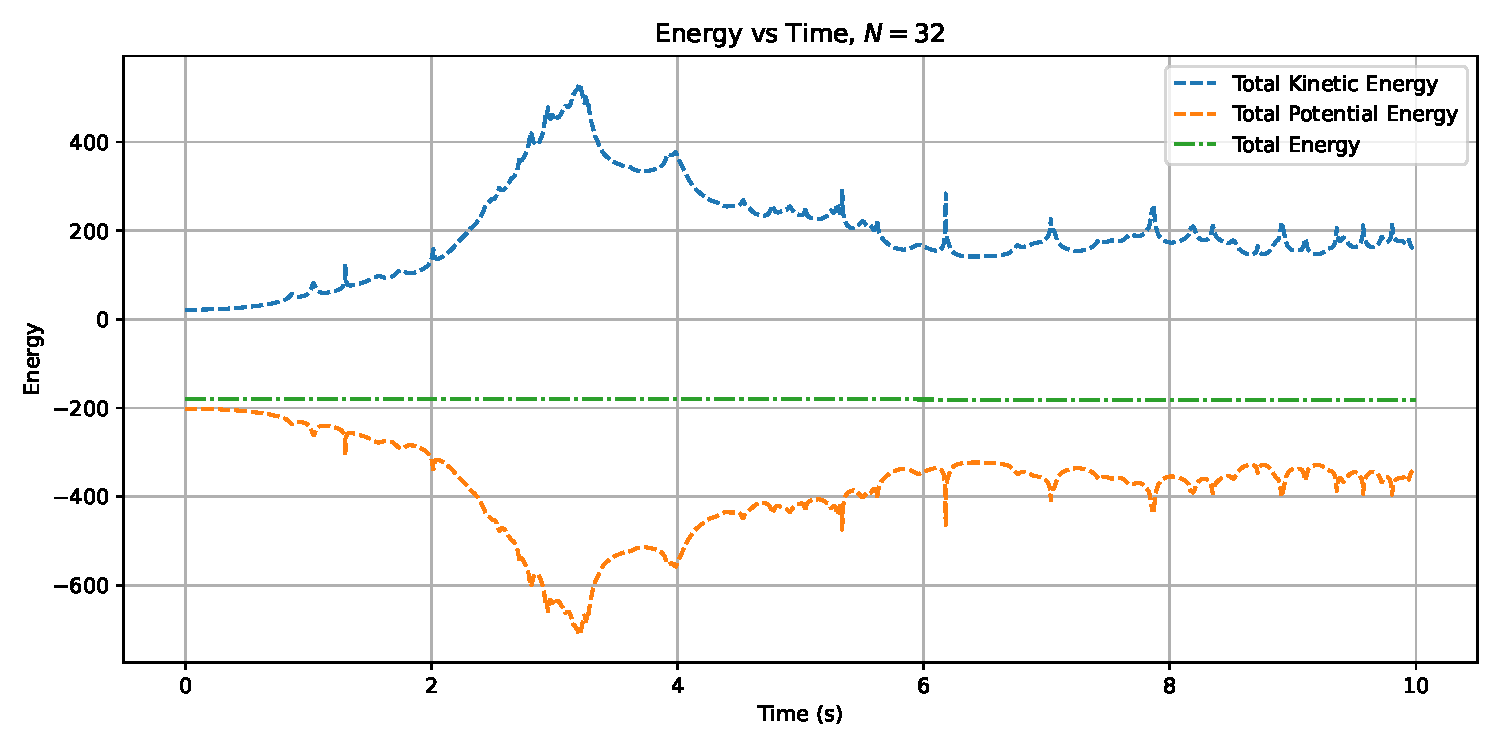
\includegraphics[height=2.0in]{../plot/cc_energy_vs_time_32_points.pdf}}
\caption{Energy v.s. Time when $n = 32$.}
\label{E-T32}
\end{figure}
\end{frame}


\begin{frame}{Results: Energy v.s. Time}
\begin{figure}
\shadowbox{
\centering
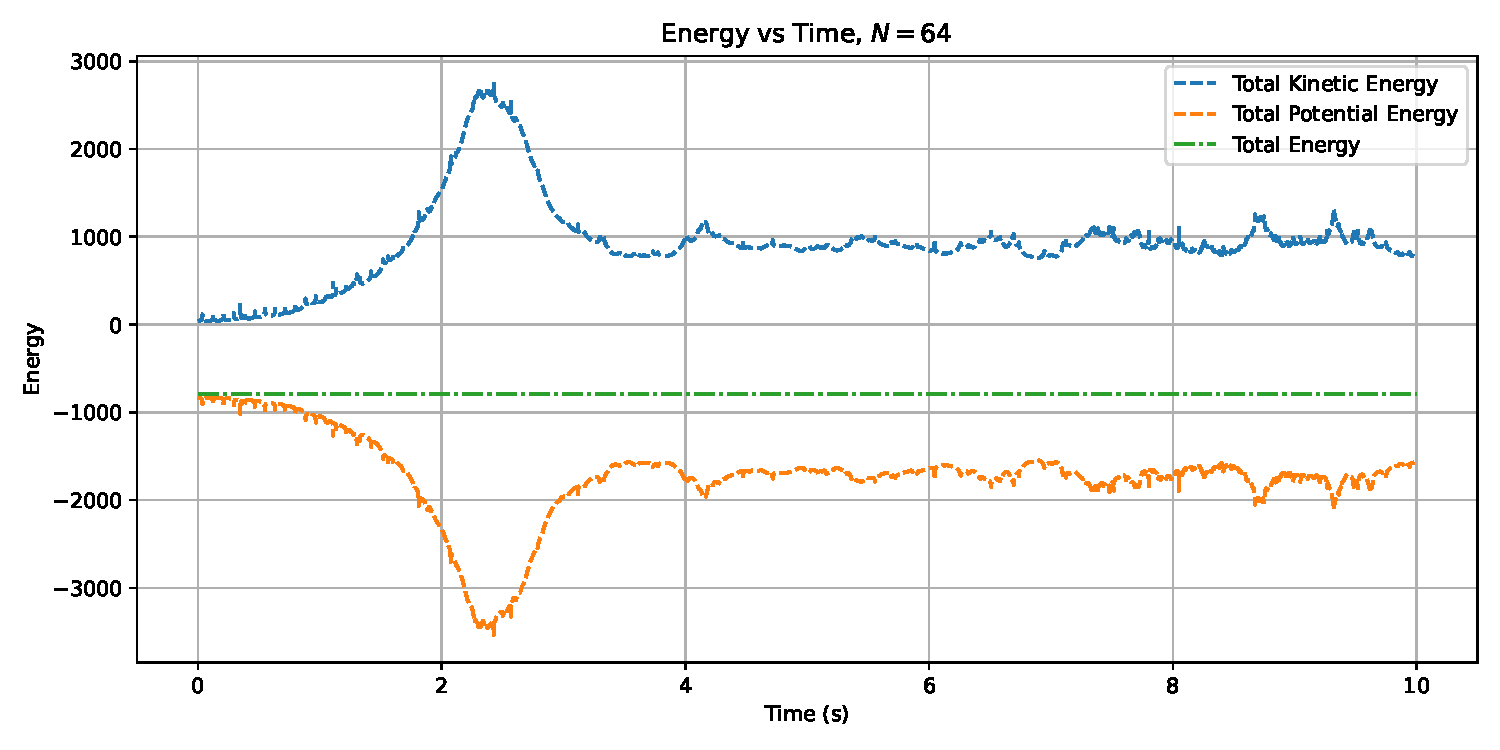
\includegraphics[height=2.0in]{../plot/cc_energy_vs_time_64_points.pdf}}
\caption{Energy v.s. Time when $n = 64$.}
\label{E-T64}
\end{figure}
\end{frame}


\begin{frame}{Results: Energy v.s. Time}
\begin{figure}
\shadowbox{
\centering
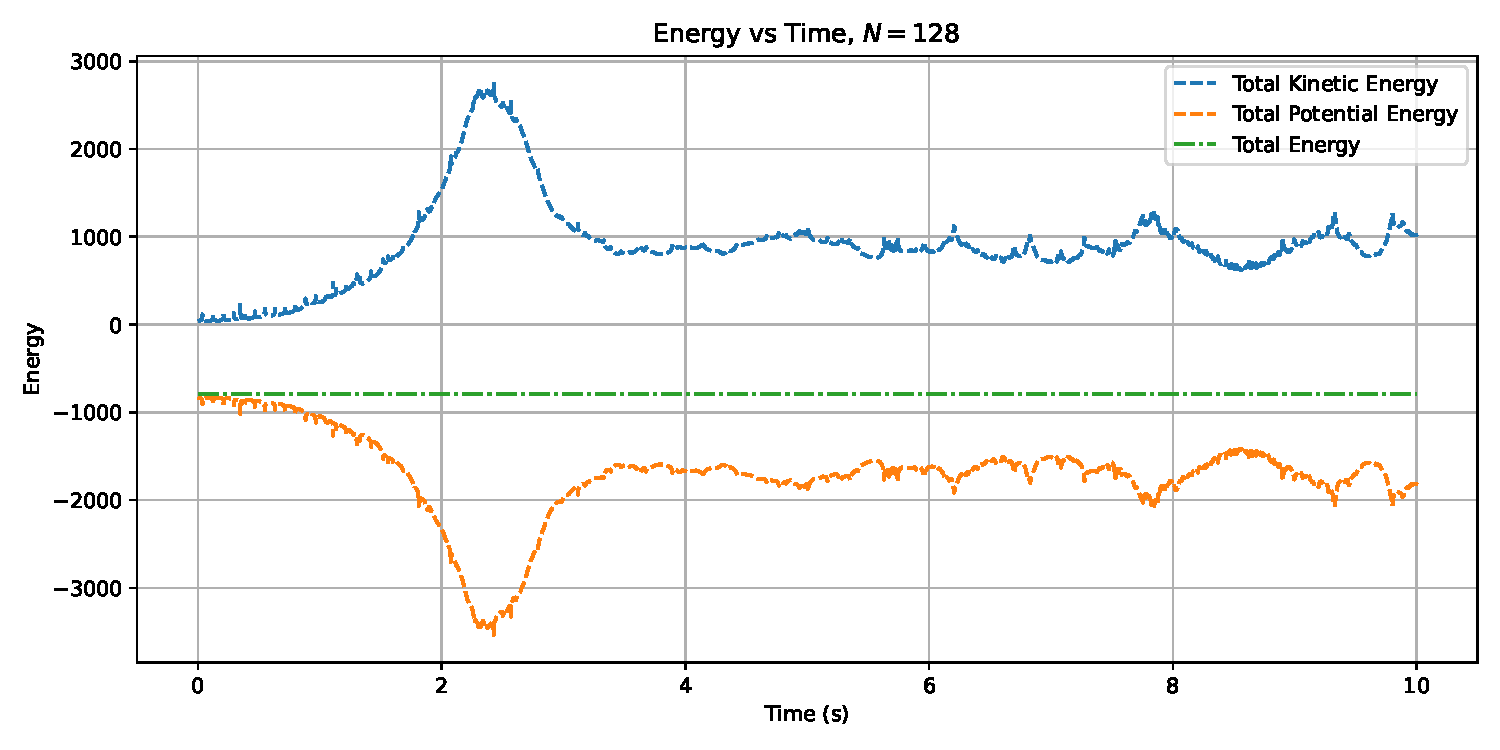
\includegraphics[height=2.0in]{../plot/cc_energy_vs_time_128_points.pdf}}
\caption{Energy v.s. Time when $n = 128$.}
\label{E-T128}
\end{figure}
\end{frame}


\begin{frame}{Results: Energy v.s. Time}
\begin{figure}
\shadowbox{
\centering
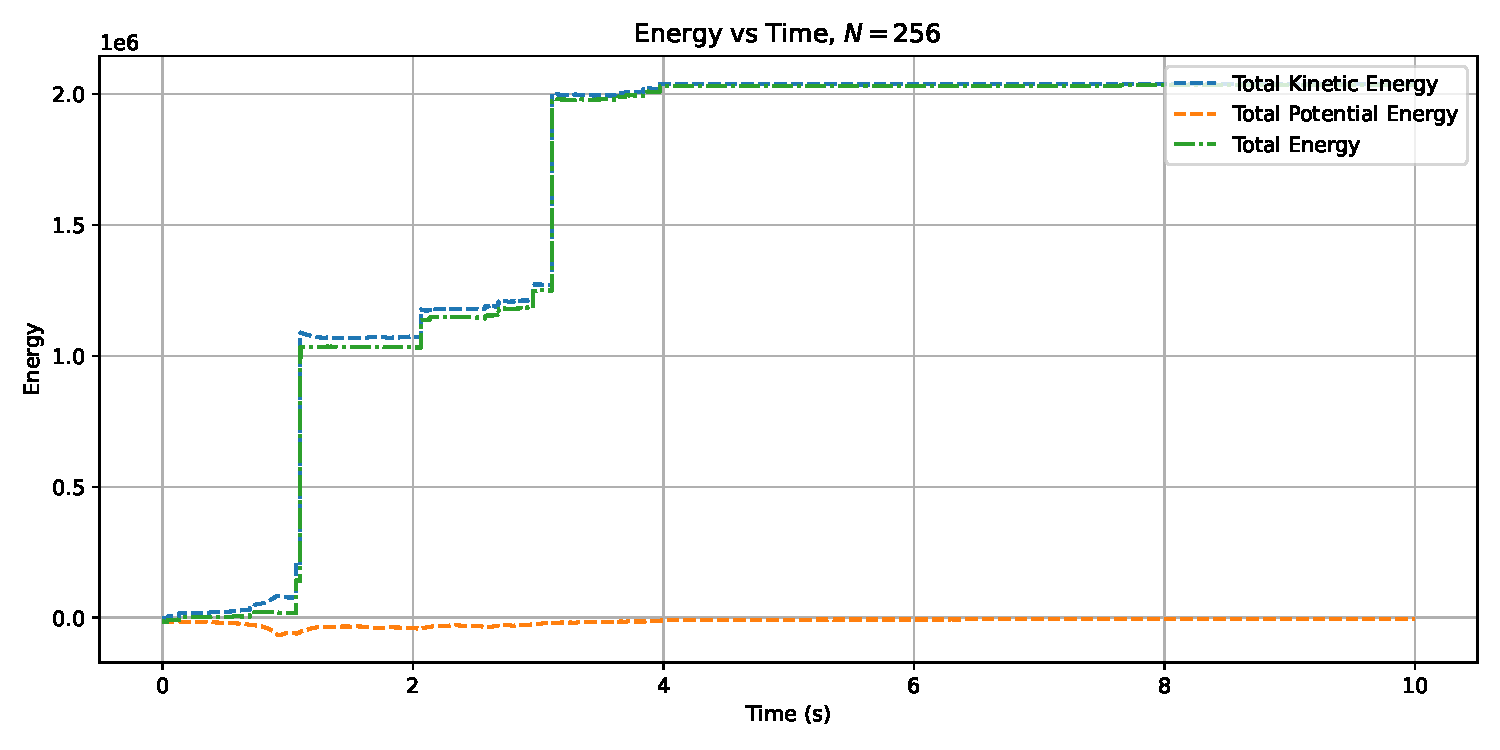
\includegraphics[height=2.0in]{../plot/cc_energy_vs_time_256_points.pdf}}
\caption{Energy v.s. Time when $n = 256$.}
\label{E-T256}
\end{figure}
\end{frame}


\begin{frame}{Results: Angular Momentum v.s. Time}
\begin{figure}
\shadowbox{
\centering
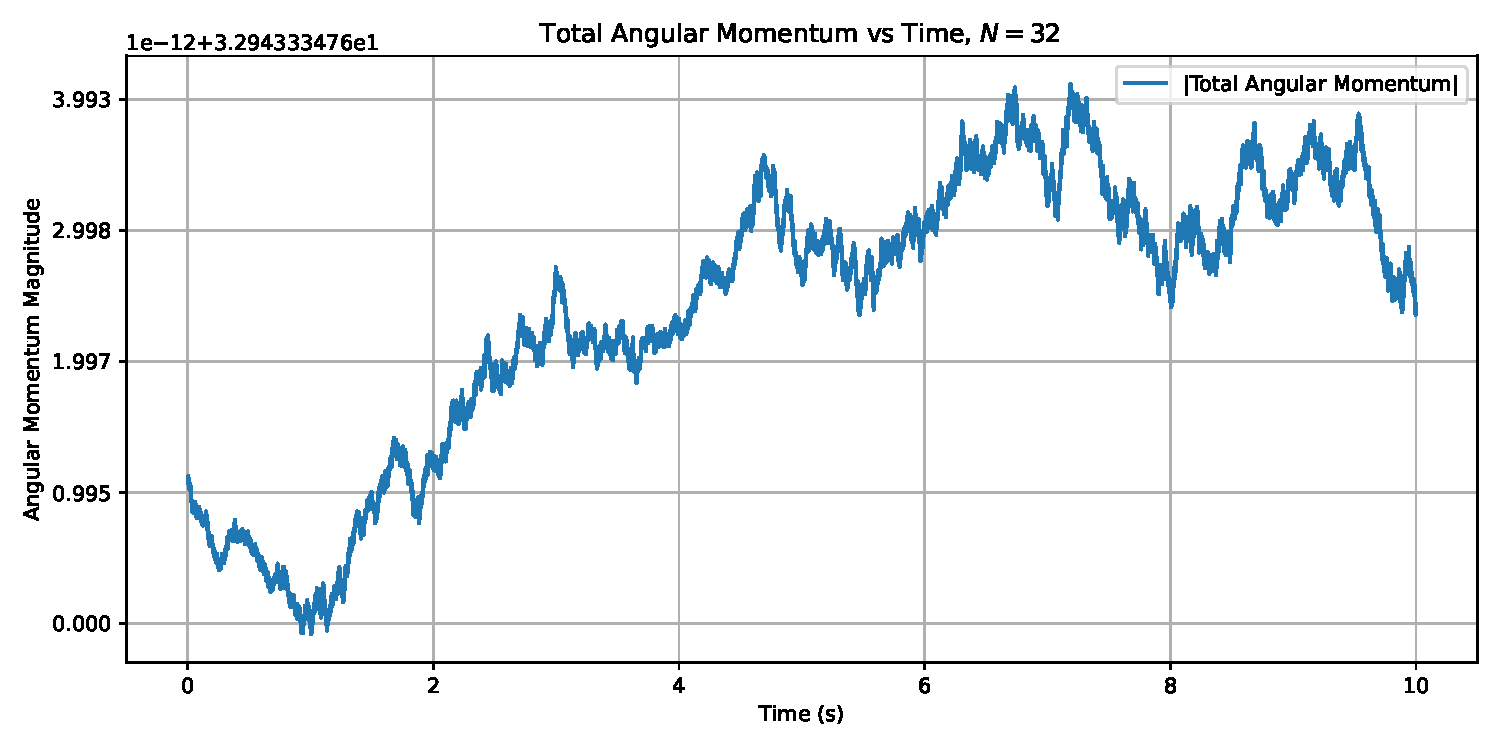
\includegraphics[height=2.0in]{../plot/cc_angular_momentum_vs_time_32_points.pdf}}
\caption{Angular Momentum v.s. Time when $n = 32$.}
\label{A-T32}
\end{figure}
\end{frame}

\begin{frame}{Results: Angular Momentum v.s. Time}
\begin{figure}
\shadowbox{
\centering
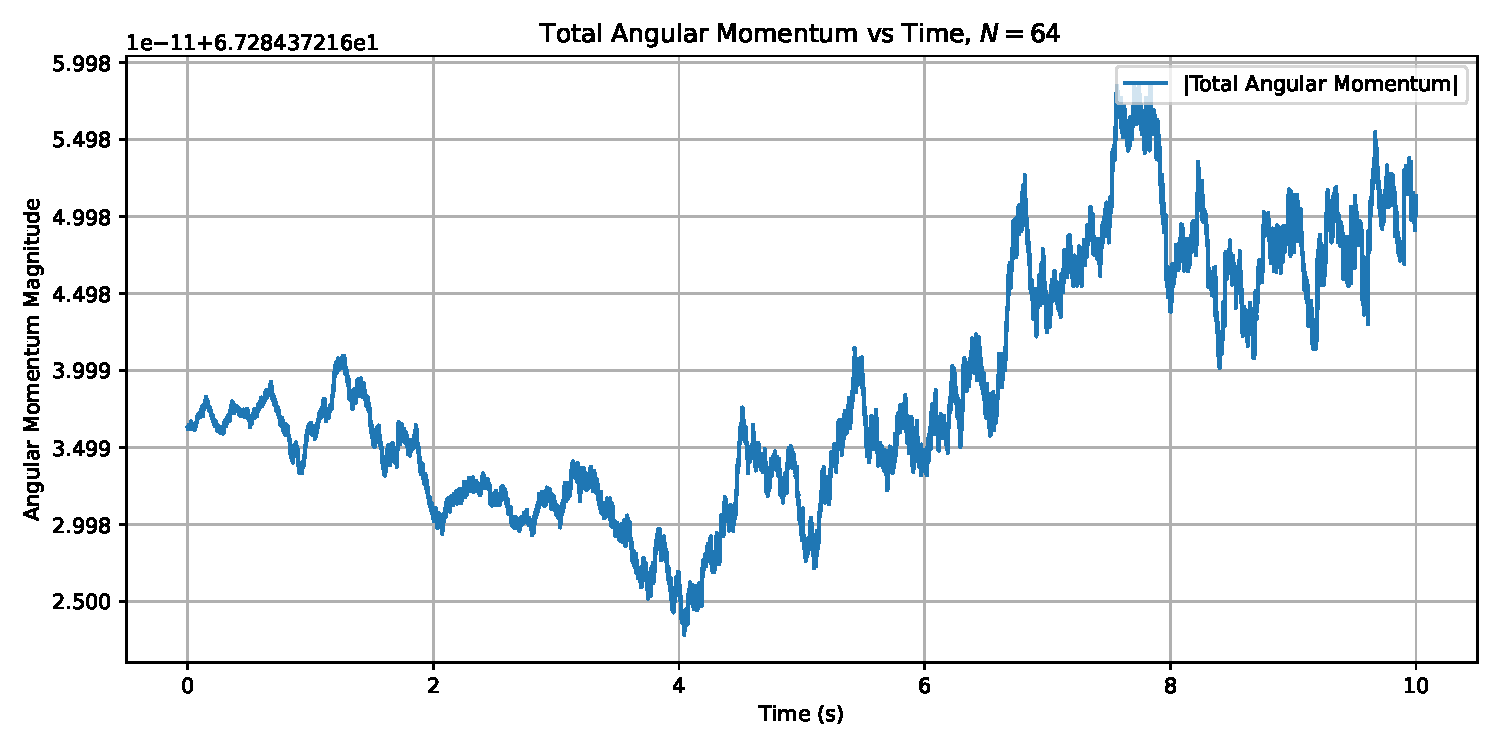
\includegraphics[height=2.0in]{../plot/cc_angular_momentum_vs_time_64_points.pdf}}
\caption{Angular Momentum v.s. Time when $n = 64$.}
\label{A-T64}
\end{figure}
\end{frame}

\begin{frame}{Results: Angular Momentum v.s. Time}
\begin{figure}
\shadowbox{
\centering
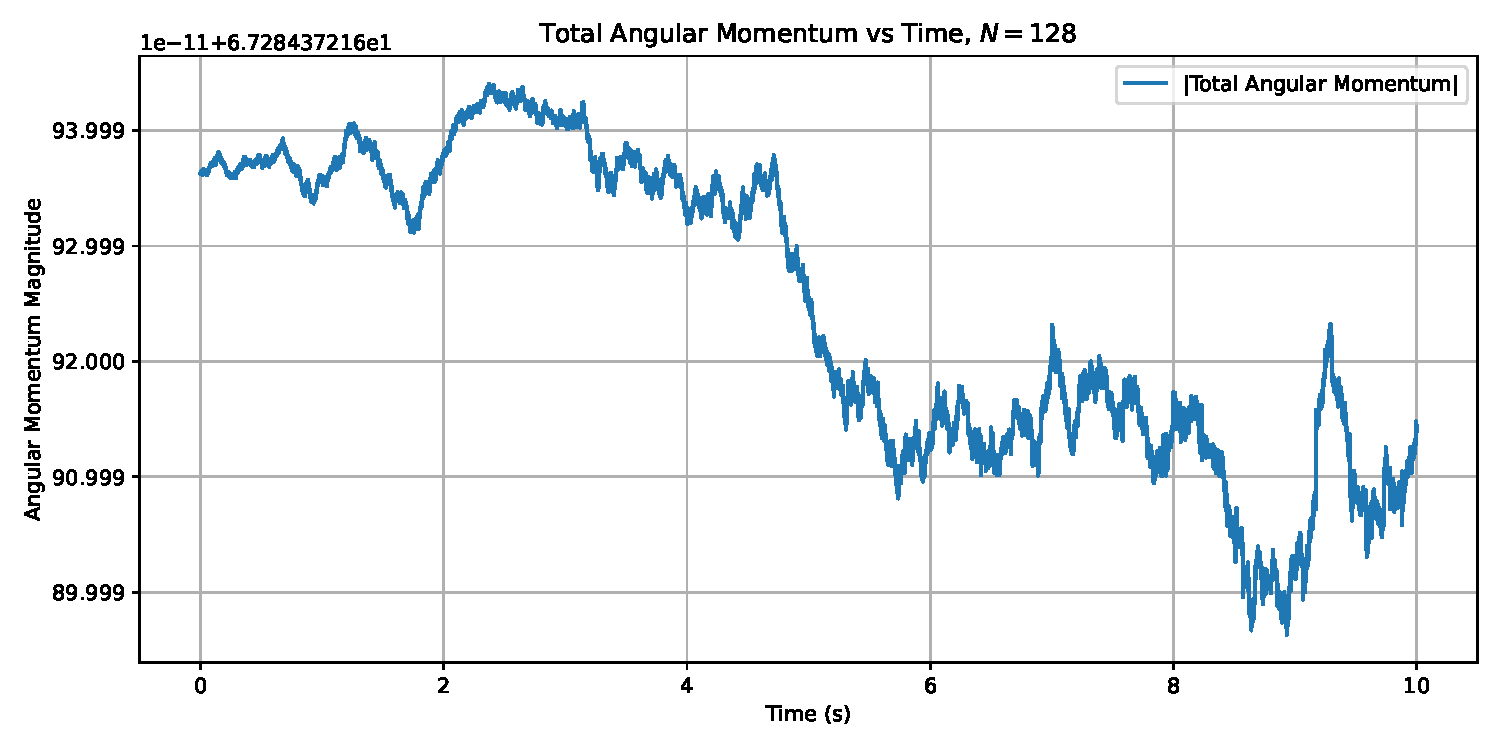
\includegraphics[height=2.0in]{../plot/cc_angular_momentum_vs_time_128_points.pdf}}
\caption{Angular Momentum v.s. Time when $n = 128$.}
\label{A-T128}
\end{figure}
\end{frame}

\begin{frame}{Results: Angular Momentum v.s. Time}
\begin{figure}
\shadowbox{
\centering
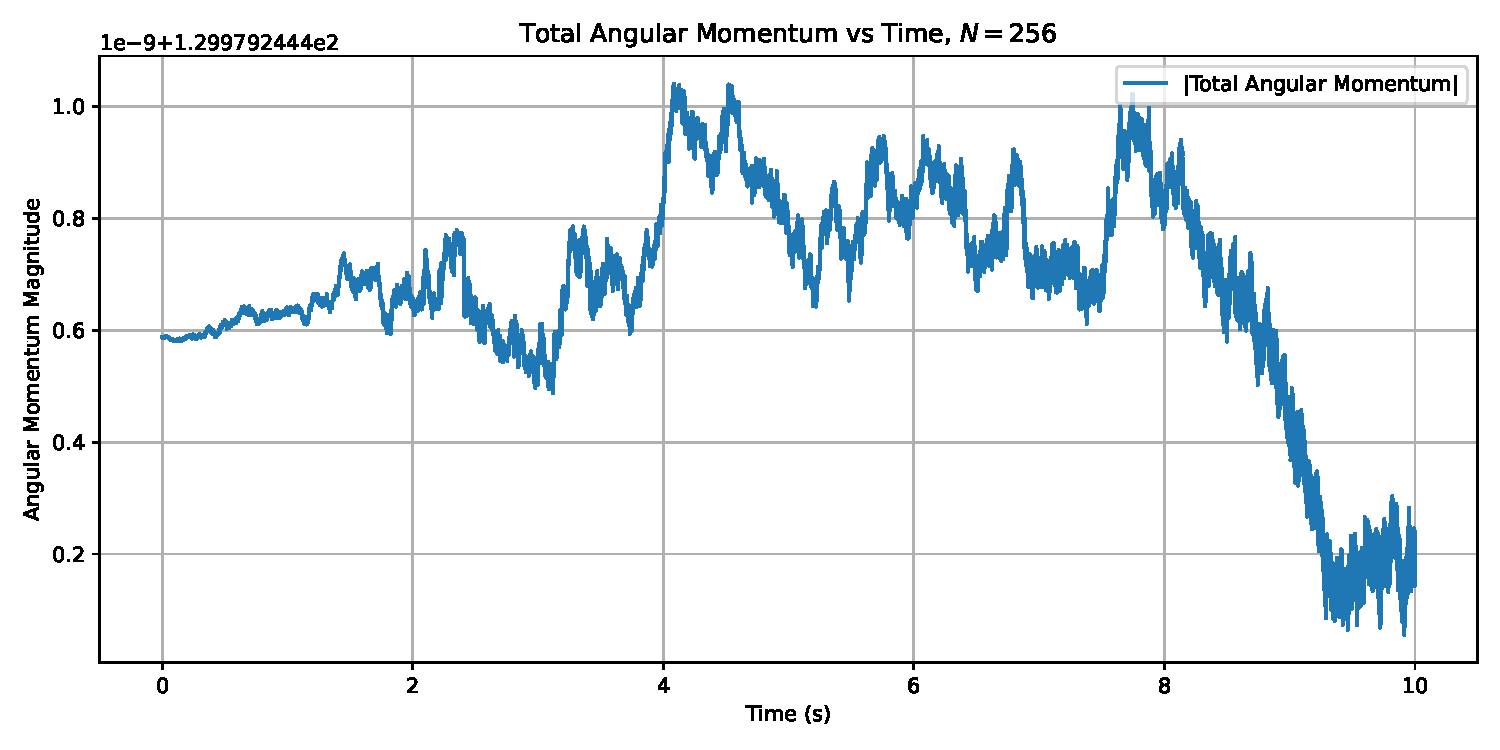
\includegraphics[height=2.0in]{../plot/cc_angular_momentum_vs_time_256_points.pdf}}
\caption{Angular Momentum v.s. Time when $n = 256$.}
\label{A-T256}
\end{figure}
\end{frame}


\begin{frame}{Results: Animation}
\url{https://www.youtube.com/watch?v=QOyjhbGaQ2A}
\end{frame}







\section{Conclusion}

\begin{frame}{Conclusion: Conservation Of Energy}
\begin{itemize}
    \item Energy conservation breaks down for $N \geq 256$.
    \begin{itemize}
        \item Happens when $N$ is large, a while after simulation.
        \item Sometimes after a large amount of collision. 
        \item Finer time-stepping can temporarily fix the issue.
    \end{itemize}
    \item Implications:
    \begin{itemize}
        \item While acceptable for small $N$, these issue may limit the suitability of the algorithm for high-precision, large $N$ studies requiring strict conservation.
    \end{itemize}
\end{itemize}
\end{frame}


\begin{frame}{Conclusion: Conservation Of Angular Momentum}
\begin{itemize}
    \item Observed very slight fluctuations in angular momentum across all $n$:
    \begin{itemize}
        \item Angular momentum conservation is much more stable than total rnergy.
        \item Possible reason is collision does not affect angular momentum.
    \end{itemize}
\end{itemize}
\end{frame}


\begin{frame}{Conclusion: Future improvements}
\begin{itemize}
    \item Future improvements:
    \begin{itemize}
        \item Implement adaptive time-stepping to better handle interactions in larger systems.
        \item Explore higher precision arithmetic to reduce numerical drift.
    \end{itemize}
\end{itemize}
\end{frame}







\section{Discussion}



\begin{frame}[fragile]{Discussion: Comparison with Actual Research}
\begin{minipage}{0.45\textwidth}

\begin{itemize}
	\item In this project, I managed to push my particle number to $N \leq 256$, but it has already been done 60 years ago.
\end{itemize}

\end{minipage}
\hspace{20pt}
\begin{minipage}{0.45\textwidth}
\begin{figure}
\shadowbox{
\centering
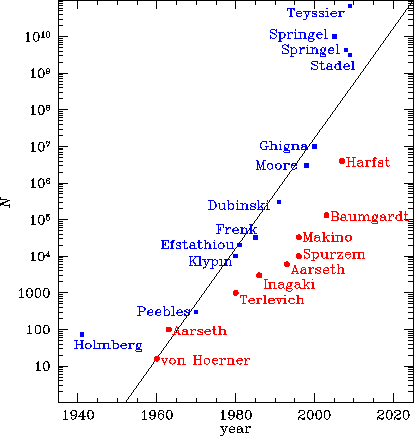
\includegraphics[width = 0.8\textwidth]{../fig/current_record.pdf}}
\caption{The increase in particle number over the past 80 years.\cite{dehnen_n-body_2011}}
\label{current-record}
\end{figure}
\end{minipage}
\end{frame}


\begin{frame}[fragile]{Discussion: Ways to Accelerate Simulation}

For many simulations, such as the \textbf{n-body}, multiple nested loops are used. And \PYTHON~Python is very slow in looping.


\begin{itemize}
	\item[\PYTHON] Use `for' loop instead of `while' loop. `for' loop is slightly faster.
	\item[\NUMBA] Use ``Numba'' decorator.
	\item[\TORCH] Harness PyTorch GPU (not so useful in I/O intensive work.)
	\item[\CC] Migrate entire project to C/C++. \checkmark
	\item[\FORTRAN] Migrate entire project to Fortran.
\end{itemize}
\end{frame}


\begin{frame}{Discussion: Ways to Accelerate Simulation}
\begin{figure}
\shadowbox{
\centering
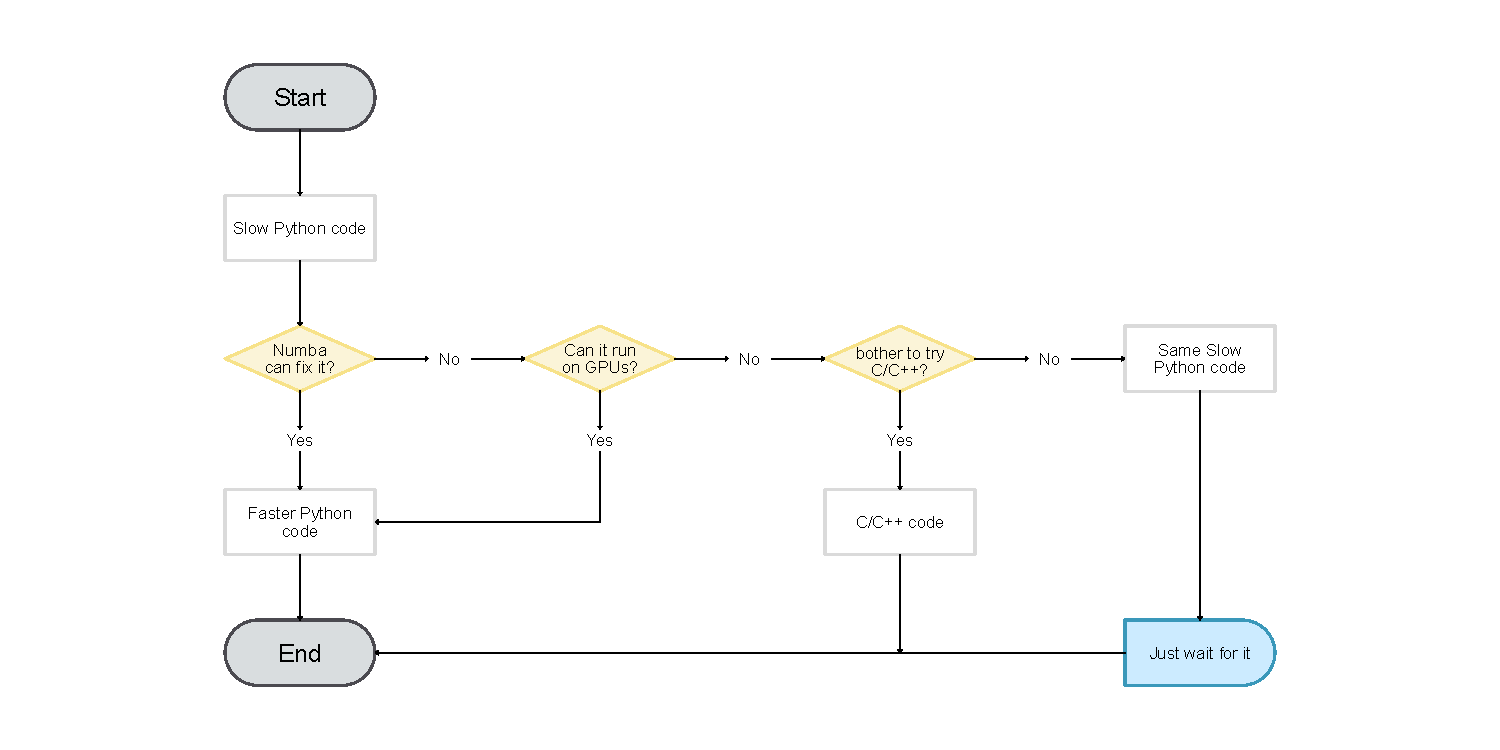
\includegraphics[height=2.0in]{../fig/FC.pdf}}
\caption{Flow chart if the Python code is slow.}
\label{FC}
\end{figure}
\end{frame}




\section{Bibliography}


\begin{frame}[allowframebreaks]{Bibliography}
\nocite{*}
\bibliographystyle{unsrt}
\bibliography{./bibliography.bib}
\end{frame}



\end{document}










Fracture energy estimates from large-scale laboratory earthquakes